%%%%%%%%%%%%%%%%%  Debut du fichier Latex  %%%%%%%%%%%%%%%%%%%%%%%%%%%%%%
\documentclass[
    a4paper, 
    12pt, onecolumn,
    %draft
]{article}

%%% Pour un texte en francais

%%\usepackage[applemac]{inputenc}
%%\usepackage[T1]{fontenc}
\usepackage[francais]{babel}
	         % encodage des lettres accentuees
%%\usepackage[utf-8]{inputenc}          % encodage des lettres accentuees

\usepackage[utf8x]{inputenc}
\usepackage[T1]{fontenc}
%\usepackage{graphicx}
%%\usepackage{graphicx} \def\BIB{}
\usepackage{multicol}
\usepackage{graphicx,wrapfig,lipsum} \def\BIB{}
\usepackage[pdftex]{hyperref}
\usepackage[round]{natbib}
\usepackage{perpage} %the perpage package
\MakePerPage{footnote} %the perpage package command
\hypersetup{
    colorlinks,%
    citecolor=black,%
    filecolor=black,%
    linkcolor=black,%
    urlcolor=blue     % can put red here to visualize the links
}

\makeatletter
\let\ORG@NAT@sort@cites\NAT@sort@cites
\def\NAT@sort@cites#1{%
  \edef\@tempa{\detokenize{#1}}%
  \ORG@NAT@sort@cites\@tempa
}
\makeatother

\makeatletter
\def\NAT@def@citea{\def\@citea{\NAT@separator}}
\makeatother

%%% Quelques raccourcis pour la mise en page
\newcommand{\remarque}[1]{{\small \it #1}}
\newcommand{\rubrique}{\bigskip \noindent $\bullet$ }

%\bibliographystyle{abbrvnat}
%\setcitestyle{authoryear,open={((},close={))}}

\renewcommand{\thefootnote}{\roman{footnote}}

\begin{document}

\bibpunct{[}{]}{,}{n}{,}{,}

%%%%%%%%%%%%%%%%%%%%%%%%%  PREMIERE PAGE %%%%%%%%%%%%%%%%%%%%%%%%%%%%%%
%%% DANS CETTE PAGE, ON REMPLACE LES INDICATIONS ENTRE CROCHETS [...]
%%% PAR LES INFORMATIONS DEMANDEES
%%%%%%%%%%%%%%%%%%%%%%%%%%%%%%%%%%%%%%%%%%%%%%%%%%%%%%%%%%%%%%%%%%%%%%%

 
\noindent GENCI\hfill \textsc{Demande d'Attribution de Ressources Informatiques}

\begin{center}
\Large  \bf
Scientific description of the project
\end{center}
\bigskip

\rubrique Title of the project : {\bf Numerical simulations of wind-accretion in \hspace*{4.42cm} high mass X-ray binary systems}
%Numerical simulation of Quasi-Periodic Oscillations in microquasars and comparison with observations

\rubrique  {\sc dari} number :
\hfill
%%% METTRE ICI LE RENSEIGNEMENTS DEMANDE
[Num\'ero de projet]

\rubrique  Scientist in charge : 
\hfill
%%% METTRE ICI LES RENSEIGNEMENTS DEMANDES
E{\sc l mellah} Ileyk


\rubrique Laboratory :  
\hfill
%%% METTRE ICI LES RENSEIGNEMENTS DEMANDES
AstroParticule \& Cosmologie (APC) - Paris 7


%%% HEURES DEMANDEES
\rubrique  Number of hours required (mono-process {\sc cpu}) :
   %%% DECOMMENTER LES LIGNES QUI CONCERNENT LE PROJET
   %%% ET REMPLACER [1200] PAR LE RENSEIGNEMENT DEMANDE
   %%% NE METTRE QUE LES DONNEES NON-NULLES
   % \newline CCRT  BULL IA64 Platine  : \hfill  [1200] heures scalaires
   % \newline CCRT  NEC SX8R Mercure   : \hfill [1200] heures vectorielles
   % \newline CCRT  BULL X\'eon Titane : \hfill [1200] heures scalaires
   % \newline CCRT  BULL X\'eon Titane : \hfill  [1200] heures CPU/GPU
   % \newline CINES IBM SP Hera        : \hfill  [1200] heures scalaires
   %  \newline CINES SGI ICE Jade       : \hfill  300\ 000 heures scalaires
   % \newline IDRIS IBM SP Vargas      : \hfill  [1200] heures scalaires
   % \newline IDRIS IBM BG/P Babel     : \hfill  [1200] heures scalaires
   % \newline IDRIS  NEC SX8 Brodie     : \hfill  [1200] heures vectorielles
     \newline CINES BULL Occigen      : \hfill  300\ 000 scalar hours

%%% RESUME
\section{Abstract}

%%% A COMMMENTER LORS DE LA REDACTION DU PROJET
%\emph{Longueur typique de {\bf 15 lignes}, longueur maximale de {\bf 1 page}.}

%The advent of high energy observation facilities in the last decades has proven the existence of powerful mechanisms emitting photons up to gamma-rays. 
%It is now commonly admitted that the most energetic events are associated with compact objects believed to be relics of massive stars. 
%These objects are prone to the most extreme gravity fields and are likely efficient attractors of the plasma present in their vicinity. 
%The motion of plasma in the close neighborhood of compact objects is only properly described in the framework of general relativistic magnetohydrodynamic (GR- MHD). 
%The equations governing GR-MHD are so complex that the only way to solve them is trough large-scale numerical simulations. 
%The topic of the present demand,  $200\ 000$ h CPU on the parallel CINES computer \lq Jade\rq\ , 
%is to sustain a computational effort dedicated to GR-(M)HD simulations of accretion flows near compact objects and to link them to synthetic observations of the 
%associated violent events.

\indent Our group is asking for  $300\ 000$ h {\sc cpu} on the parallel {\sc cines} computer \lq Occigen\rq\ so as to investigate phenomenological statements concerning wind accretion in Supergiant High Mass X-ray Binaries (Sg-{\sc hmxb}), whether they host a neutron star or a black hole. We developed a specific approach to describe both the large scale ballistic behavior of the stellar companion wind to the accretion radius of the compact object (whom ratio is typically of the order of 10$^{-1}$) and then, down to a few hundreds of gravitational radii (whom relative size compare to the former ranges from 10$^{-3}$ to 10$^{-5}$). The huge dynamical spatial scale is made possible thanks to both the highly parallelized {\sc mpi-amrvac} software and to a stretched grid centered on the compact object. The former program makes it possible to grasp shocks and non axisymmetric instabilities likely to give birth to potentially transient accretion discs around the compact object. The three-dimensional characterization of such flows is a crucial prerequisite to better appreciate both the expected X-ray time variabilites and the initial conditions from which close-in accretion discs ought to be modeled. \\

\newpage\section{General presentation}

%%% A COMMMENTER LORS DE LA REDACTION DU PROJET
%\emph{Longueur typique {\bf 2 pages}, longueur maximale de {\bf 4 pages}. Si le projet se d\'ecompose en sous-projets, {\bf 2 pages additionnelles maximum par sous-projets}.}
%\vskip 0.2cm  
%\emph{Cette partie doit montrer l'int\'er\^et scientifique du projet. Le canevas suivant est propos\'e : 
%pr\'eciser les objectifs,
%situer les travaux de l'\'equipe sur le th\`eme de recherche propos\'e tant vis \`a vis du travail d\'ej\`a  
%effectu\'e par l'\'equipe (r\'esultats acquis sur le sujet), que vis \`a  vis d'autres travaux sur un plan national
%et international,
%donner une liste de publications de l'\'equipe dans le domaine dans la section \ref{Sec:Biblio}. On peut joindre au dossier tous les documents (en format pdf) annexes jug\'es utiles.}

\indent The number of detected Sg-{\sc hmxb} has dramatically increased as the recent space missions stretched the limits of the high energy part of the light spectrum \citep{Liu2006}. Once believed to be rare \citep{Illarionov1975}, those X-ray luminous wind-fed compact objects orbiting an evolved {\sc O}/{\sc B} star turned out to not fit well in the previously sketched categories. The characterization of the companion star is usually a challenge in itself because of the high obscuration of those systems, lying close from the Galactic plane and kiloparsecs away from us, but the recent inflation of the number of extragalactic {\sc hmxb} partly lifted this difficulty. Still, the main information we get from those objects (some being microquasars whom study is believed to enrich our understanding of Active Galactic Nuclei) comes from the X-ray emission to which they owe their name.\\
\begin{table}[h]
\centering
\begin{tabular}{||c|c|c||}
\hline\hline
Names & Status & Laboratory \\\hline
EL MELLAH Ileyk & Doctorant & APC\\ \hline 
CASSE Fabien & Ma\^itre de conf\'erence & APC \\ \hline
DODU Fabrice & Ing\'enieur de recherche &APC \\ \hline
\hline\hline
\end{tabular}
\caption{Members of the collaboration}
\end{table}

\indent This hard radiation, whom discovery in 1962 \citep{Giacconi1962} brought up so many questions, remains puzzling when one attempts to explain the different "families" of behaviors observed - if that an agreement is found on the very classification. Those complex systems have been dissected (the launching of the stellar wind, its orbital trajectory, the shocks it can form, its subsequent accretion onto the compact objects, etc) but in order to go beyond toy-models which set the asymptotic separated behaviors, one needs to tackle the entire fate of the stellar material, from the clumpy wind scale down to the close vicinity of the compact object (being, in our study, around a hundred gravitational radii for a black hole and the magnetosphere scale for a neutron star). For instance, being able to corroborate the identity of the compact object deduced from orbital considerations would bring more scientific weight to the current observational constraints on the equation of state of matter in neutron stars. So as to achieve such assessment, one must first wonder how the orbital parameters (the orbital period, the mass of the compact object, the mass ratio, the eccentricity) and the properties of the stellar companion (its wind velocity and clumpiness, its mass ejection rate) prescribe the compact object environment to disentangle the contingent from the essential causes. Independently from the accreting body nature, the systems we intend to model already differ a lot from each other :\\
\begin{itemize}
\item \textbf{Cyg X-1 :} it hosts a highly R{\sc oche} lobe deformed \citep{Avni1975} Sg star \citep{Shenavrin2011} orbiting a compact object of comparable mass every 5.6 days. Although one of the most studied {\sc hmxb} - if not the most - its genericity remains suspicious.\\
\item \textbf{LMC X-1 :} this extragalactic close X-ray binary presents a peculiar Onfp class \citep{Walborn2010} star whom rapid rotation might transfer an important amount of stellar angular momentum to the wind. \\
\item \textbf{Vela X-1 :} the archetype of the Sg-{\sc hmxb}. Characterized by a larger mass ratio than the two previous ones, this eclipsing system feeds its compact object through the specially intense stellar wind of its B stellar companion, well embedded in its R{\sc oche} lobe.\\
\item \textbf{4U 1907+09 :} in this high mass ratio eccentric X-ray binary, a hybrid accretion might proceed, mixing R{\sc oche} lobe overflow and wind accretion. The torque accreted matter exerts on the compact object has been reported to potentially alternate between positive and negative values.\\
\end{itemize}

\begin{wrapfigure}{l}{6cm}
%\caption{A wrapped figure going nicely inside the text.}
\vspace*{-23pt}
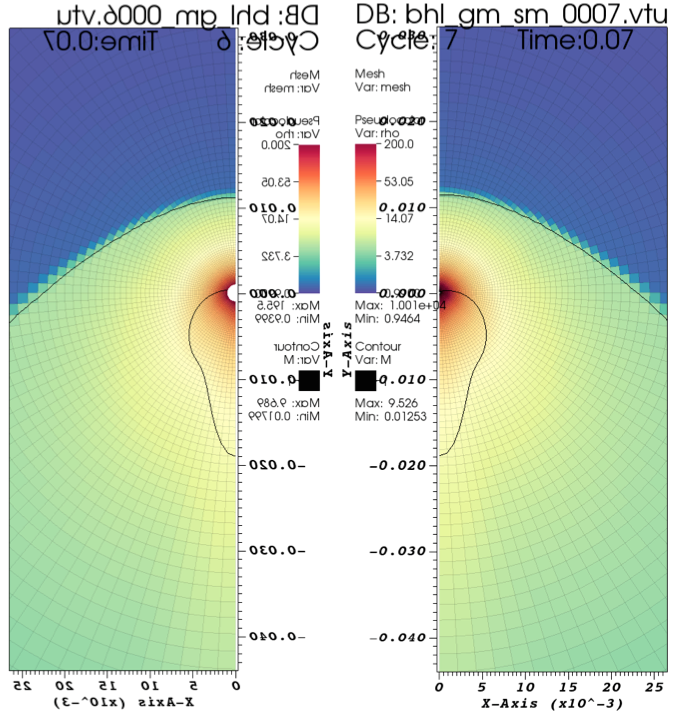
\includegraphics[height=7cm, width=6cm]{shock_independent_inner_boundary_size}
\caption{Bow shock and sonic surfaces of an axisymmetric 2.5D accretion flow. Notice the stretched grid}
\label{fig:bow2.5d}
\vspace*{-23pt}
\end{wrapfigure} 

\indent B{\sc ondi}, H{\sc oyle} and L{\sc yttleton} laid the foundations of an understanding of axisymmetric accretion flows (see the review \citep{Edgar:2004ip}) like the one we started from as a numerical sanity check (see next paragraph). Their ballistic approach has been improved to account for pressure effects \citep{Horedt2000}, making the accretion line in the wake of the accreting body an accretion tail. In the end of the 80's, two dimensional simulations of those flows \citep{Matsuda1987,Fryxell1988} revealed an instability, coined the flip-flop one ; the two dimensional cylindrical geometry, the low resolution and the oversized inner boundary compare to the actual size of the accretor made this instability suspicious to the community, until theoretical models \citep{Foglizzo2005} supported the possibility of an instability growth important enough to account for the formation of tiny and transient discs around the accretor. The issue has remained polemical up to nowadays as the computational capabilities have proven insufficient to grasp the whole problem. That is why we developed a reliable upwind scheme on a logarithmic three dimensional grid centered on the accretor to jump from large to small scales at a cheaper computational cost. However, this numerical swindle would not have been enough to beat the dynamics barrier without the highly parallelized structure of the finite volumes program {\sc mpi}-{\sc amrvac}. Using the two together, we have now good hope to make the inner boundary small enough to be whether physical (for neutron star systems) or transparent (for black hole systems). The Figure\,\ref{fig:bow2.5d} shows for instance a simulation where the structure of the flow and of the sonic surface is not altered by the unphysical inner boundary.\\

 \begin{figure}[h]
 \centering
 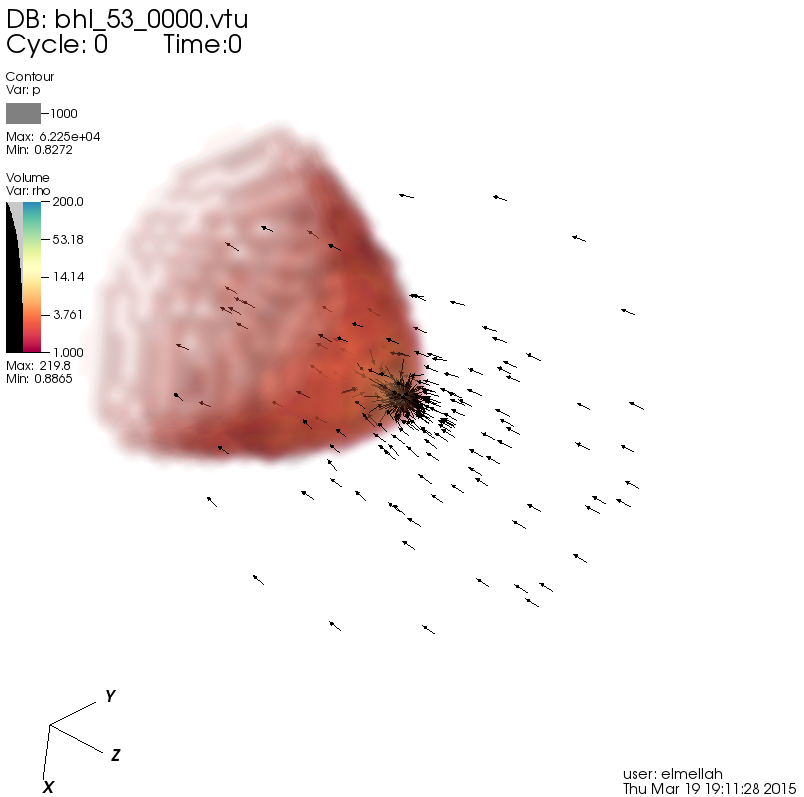
\includegraphics[width=9cm]{3D_initial_setup}  
 \caption{3D initial setup deduced from the relaxed 2.5D one}
 \label{fig:relax}
 \end{figure}
 
\indent Concerning the numerical reliability of our setup, we already validated the behavior of the gas in 2.5D spherical geometry within the accretion radius by showing that the axisymmetric configuration is in agreement with semi-analytical results derived by \citep{Foglizzo1996}, especially regarding the topology of the sonic surface for a detached bow shock. Nevertheless, in order to enable the possible non axisymmetric instabilities to develop and to consider more realistic outer boundary conditions, we still need to free those 2.5D numerically relaxed simulations from their constraining geometry and go for the full 3D configuration. The computational time it requires motivates our application to the {\sc cines} facilities.\\
\indent It is noteworthy that our work also aim to help constraining future and incoming observational mission (\href{http://www.the-athena-x-ray-observatory.eu}{{\sc athena}} \& \href{http://astro-h.isas.jaxa.jp/en/}{{\sc astro-h}} eg) : which waveband should we look after? Which time scale should we aim to characterize processes involved in the building up of an accretion disc? Since the mass accretion rate determines the available power convertible into X-ray luminosity, such simulations would also set lower limits for the sensibility required to probe events taking place in the very neighborhood of the compact object. The related studies, led in parallel, of the instabilities in this strong gravitational field regims (the {\sc nova}s project eg) might, one day, tell us more about the Physics at stake in those extreme environments : what kind of hitherto unseen events can take place in the wildness of a neutron star light cylinder or of a black hole ergosphere?

\section{Method}

%%% A COMMMENTER LORS DE LA REDACTION DU PROJET
%\emph{Cette partie doit \^etre suffisamment pr\'ecise et argument\'ee pour permettre au Comit\'e Th\'ematique d'appr\'ecier 
%l'ad\'equation de l'architecture
%pr\'evue (scalaire, vectorielle ou parall\`ele, GPU ...) au probl\`eme pos\'e. Il convient aussi de justifier clairement la n\'ecessit\'e de l'utilisation d'un tr\`es grand \'equipement pour le traitement informatique du projet.
%Voici une proposition de plan (\`a adapter selon le sujet) :
%Algorithme utilis\'e, adaptation \`a la plate-forme vis\'ee; Modalit\'es d'optimisation (vectorisation, optimisation superscalaire, parall\'elisation); Structure du programme; Logiciels n\'ecessaires; Langages utilis\'es; Biblioth\`eques pr\'evues; Syst\`emes de gestion de bases de donn\'ees ou syst\`emes documentaires utilis\'ees.}


\subsection{Numerical tools}

%%% A COMMMENTER LORS DE LA REDACTION DU PROJET
%\emph{Longueur typique de  {\bf 4 pages}, longueur maximale de {\bf 6 pages}.}

\subsubsection*{The \textbf{\textsc {mpi-amrvac}} code}

\indent The code {\sc mpi-amrvac} \citep{Porth:2014wv} (Message Passing Interface - Adaptative Mesh Refinement Versatile Advection Code) is an {\sc amr} code parallelized with Open{\sc mpi}. This code was developed to solve {\sc hd} and {\sc mhd} hyperbolic conservative equations, whether in a classical or a relativistic framework. The user-defined additional source terms\footnote{Radiative cooling (in optically thick or thin regims), gravity, viscosity...} entitle to explore a wide range of physical one or two-fluids configurations. Several types of R{\sc iemann} solvers are implemented (R{\sc oe} and H{\sc arten}-L{\sc ax}-V{\sc an} L{\sc eer} ones eg), along with flux-limiter schemes as the Total Variation Diminishing ({\sc tvd}) ones.\\
\indent The {\sc amr} grid structure is based on the use of sub-grids (of a few tens of cells in every dimension) in a tree architecture (octree in 3D). At each iteration the code uses an internal L{\sc ohner}'s method or user-supplied criteria to determine if a sub-grid needs to be refined, left as it is, or unrefined. The tree structure replaces each refined sub-grid by a $2^D$ sub-grid of the same cell-size but with the area of each cell less by a factor $2^D$. For the present project, we will probably not use the {\sc amr} but instead, we designed a non-regular grid fitting the geometry of the system and enabling us to reach outer radius to inner radius ratio up to $10^5$ at a low computational cost. The grid is designed to maintain the same radial to azimuthal cell size ratio constant for any radius of the simulation. The smallness of the cells close to the inner boundary sets the C{\sc ourant}-F{\sc riedrichs}-L{\sc ewy} ({\sc cfl}) time step to such small values that several tens of millions of iterations are expected in order to describe the flow dynamics both at large and small scales. Such computation can only be achieved using the large number of {\sc cpu} available on supercomputers.
\newline

 \begin{figure}
\centering
 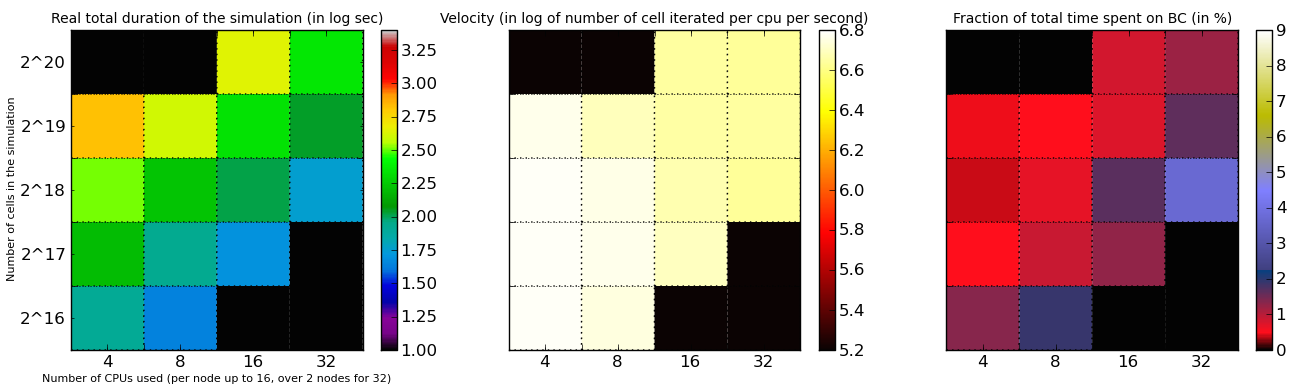
\includegraphics[width=14cm,height=5cm]{Scaling_node_14_15_unthreaded.png} 
 \caption{General scaling of the MPI-AMRVAC code performed on the Fran\c cois Arago Center ({\sc fac}e) cluster at Paris 7 Diderot} 
 \label{fig:scaling_FACe}
\end{figure}

\subsubsection*{Parallelization and scaling}
\begin{wrapfigure}{r}{6cm}
\vspace*{-60pt}
%\caption{A wrapped figure going nicely inside the text.}
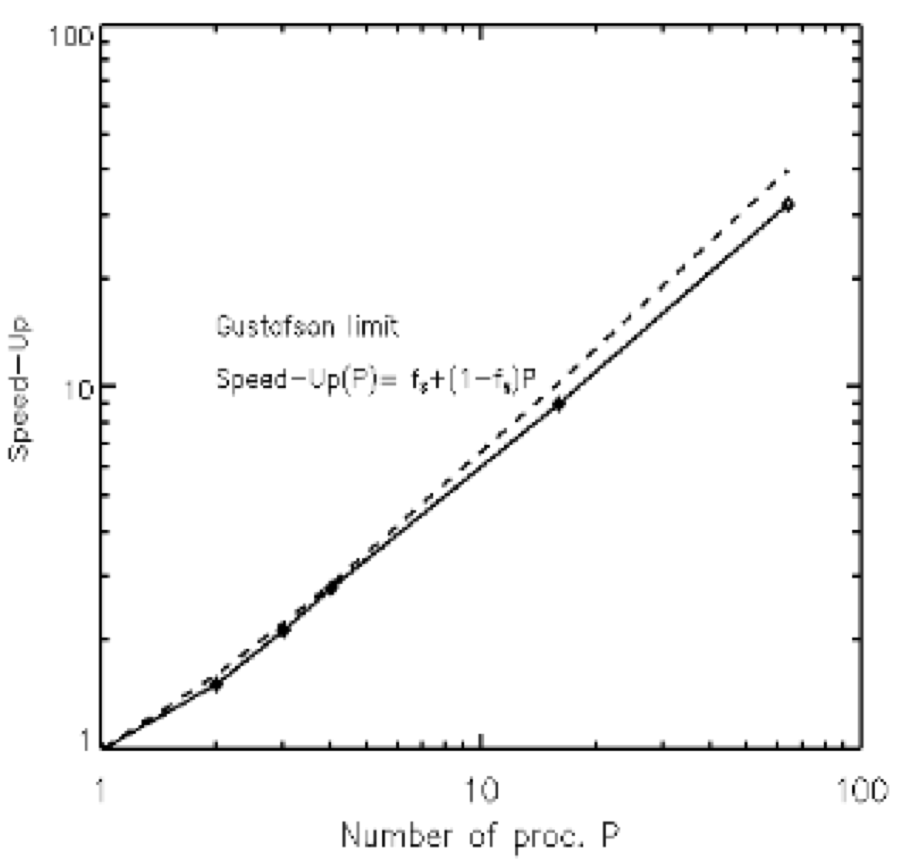
\includegraphics[height=6cm, width=6cm]{scaling_1}
\caption{Scaling of the MPI-AMRVAC code performed on the JADE super-computer}
\label{fig:scaling_JADE}
\end{wrapfigure} 
\indent The parallelization relies on Open{\sc mpi} libraries and the scalability test done on \lq Jade\rq  by Zakaria M{\sc eliani} has showed an efficiency of the order of 80\% on 2000 processors (see Figure\,\ref{fig:scaling_JADE}). This value is very close to the theoretical limit when one takes into account the I/O of the code needed to write the data. Those results of the parallelization efficiency were obtained using a test case in relativistic hydrodynamics, taking into account the propagation of shocks with Lorentz factors between 100 and 1000. The main test was done in 2D with 10 levels of {\sc amr} with a refinement ratio of 2. This allowed us to locally increase the resolution of the simulation by a factor of $218$. The {\sc mpi-amrvac} code also includes two different methods to write the data allowing a better flexibility. Indeed, {\sc mpi-amrvac} can either use the method  MPI-II/IO or the method that consists of sending all the data from the slave node to the master node to minimise the number of processors taking part in the writing.

\subsection{Time justification}

\indent If the logarithmically stretched grid we developed enables us to investigate this intrinsically multi-scale problem at an affordable cost, the huge time dynamics entailed precludes extended numerical simulations on local clusters as the \href{http://www.apc.univ-paris7.fr/FACe/en/cluster-arago}{{\sc fac}e} one (see Figure\,\ref{fig:scaling_FACe}). The initial 2.5D relaxation step (cf Figure\,\ref{fig:relax}) partly lifts this caveat but for non axissymmetric outer boundary conditions, we still require the computational ability to monitor the flow over large scale time scales, which implies dozens of 10$^6$ iterations.\\
\indent Here would be the main use of the 300 000 {\sc cpu} hours :\\
\begin{itemize}
\item[$\star$] \textbf{10 kh$\cdot$\textsc{cpu}} to definitely confirm the observed trend of Figure\,\ref{fig:bow2.5d} concerning the sonic surface shape of an axisymmetric flow, by making the inner boundary small enough to reach the physical size of the compact object. This simulation would firmly validate the theoretical approach suggested by \citep{Foglizzo1996} to semi-analytically study those flows.
\item[$\star$] \textbf{30\footnote{30 points to explore the two dimensional ($M_{\infty}$,$M$) space} $\times$ 300 h$\cdot$\textsc{cpu} $\sim$ 10 kh$\cdot$\textsc{cpu}} to explore the dependency of the stationary shock properties with the M{\sc ach} number $M_{\infty}$ and the mass of the accreting body $M$ (attached/detached shocks, position of the forefront, opening angle of the tail, transverse density profile...).
\item[$\star$] \textbf{4 systems $\times$ 7 possible configurations\footnote{Depending on the wind velocity, its clumpiness, its temperature, the orbital parameters...} $\times$ 10 kh$\cdot$\textsc{cpu} $\sim$ 280 kh$\cdot$\textsc{cpu}} to decide between different observationally deduced system properties and retroactivally, to shed light on the relevant large scale phenomenological description among all those which led observers to different conclusions.\\ 
\end{itemize}
\indent \indent Eventually, this numerical simulations set as a whole would bring fruitful answers to our core problematics : to what extent orbital parameters and properties of the stellar companion constrain the vicinity of the compact object in a wind-fed {\sc hmxb}? Such answers would be robust starting points to inspire instability studies in those systems.

%une simulation en moyenne se compte en jour, avec  entre 64 et 512 proc...
%   256 proc pendant 24h: 5000...   
%   donc 10jours de simu, a notre niveau actuel va nous permettre d'avancer... et si besoin redemande en juin
%   


%\subsection{Justification de l'emploi de la machine demand\'ee}

%%% A COMMMENTER LORS DE LA REDACTION DU PROJET
%\emph{Longueur typique de {\bf 1 page}, longueur maximale de  {\bf 2 pages}.}

\newpage

\section{Bibliographie}
\label{Sec:Biblio}
 
\bibliographystyle{plainnat}
\bibliography{/Users/ielm/Documents/Bibtex/proposal_DARI_Ap_15}

\end{document}
%%%%%%%%%%%%%%%%%  Fin du fichier Latex  %%%%%%%%%%%%%%%%%%%%%%%%%%%%%%

